
\chapter{Einführung}
\label{ch:Introduction}
Der Aufstieg des Cloud Computing ermöglicht Kunden ihre Applikationen dynamisch zu skalieren. Dies steigert nicht nur die Verfügbarkeit für den Endnutzer, sondern hat auch ökologische und ökonomische Vorteile. Investitionen in Hardware und Software können reduziert werden, da die Ressourcennutzung durch das dynamische Skalieren optimiert wird. Gleichzeitig kann der Klimafußabdruck reduziert werden, da Ressourcen nicht unnötig brach liegen \cite{ASurveyOn} \cite{ReviewOfAtuoScaling}. \\
Trotz dieser Vorteile ist es eine nicht triviale Aufgabe, die korrekte Allokation von Ressourcen zu planen, vorherzusagen und auszuführen. Gründe dafür sind die verschiedenen Charakteristiken der Workloads im Cloud Computing, wie beispielsweise Varianz, Periodizität (Muster, die sich täglich, wöchentlich etc. wiederholen), Art der benötigten Ressource oder Änderungsrate \cite{PEAS}. \\  
Diese Aufgabe wird mittels Auto-Skalierer durchgeführt, die basierend auf der Systemlast, diversen Metriken und Strategien dynamisch Ressourcen hinzufügen oder wieder wegnehmen. Zwischen dem Cloud Service Anbieter und dem Kunden existiert dabei ein Rahmenvertrag (Service Level Agreements oder kurz, \textit{SLAs}), der die Dienstgüte des Cloud Service beschreibt \cite{ASurveyOn}. Dieser Vertrag beschreibt Qualitätsparameter wie Verfügbarkeit, Reaktionszeit des Anbieters, Durchsatz oder die Ausfallrate der Infrastruktur. Der Auto-Skalierer sollte dabei so arbeiten, dass er diese Parameter erfüllt und dabei die Gesamtkosten gering hält, sodass der Anbieter mit seiner angebotenen Leistung Profit erzielen kann. \\
In den letzten Jahren wurden deswegen verschiedenste Strategien für Auto-Skalierer entwickelt, die diese Aufgabe effizient lösen sollen \cite{ReviewOfAtuoScaling}. Um konkrete Implementierungen dieser Auto-Skalierer zu evaluieren, kann man diese auf realer Infrastruktur und unter einer gegebenen Last testen. Dies jedoch erfordert hohe Kosten, da eine Infrastruktur bereitgestellt und eine Last erzeugt werden muss, um so das Verhalten des Auto-Skalieres zu beobachten. Bei einer Simulation hingegen können diese Kosten größtenteils reduziert werden, da nur Ressourcen für die Durchführung der Simulation benötigt werden.\\
Um eine solche Simulation durchzuführen muss eine Umgebung geschaffen werden, in der die Infrastruktur eines Cloud-Service Anbieters modelliert wird, um so das Verhalten eines gegebenen Auto-Skalierers zu beobachten. Diese Entwicklung einer solchen Umgebung, auch Testbench für Auto-Skalierer genannt, ist der Bestandteil dieses Praktikums und wird in der folgenden Dokumentation beschrieben.


\section{Motivation}
\label{sec:Introduction:Motivation}
Bei einer zeit-diskrete Simulationen ist es möglich, das Verhalten eines Auto-Skalierers anhand einer gegebenen diskreten Last auf einer simulierten Infrastruktur zu testen. Dabei kann die diskretisierte Last sowohl auf einer realen Last basieren, die über einen sehr langen Zeitraum gemessen wurde, als auch auf einer generierten Last, die verschiedene, der in der Einführung beschriebenen Charakteristika aufweist. Es ist daher möglich, den Auto-Skalierer ohne größere Anstrengungen unter verschiedenen Lastbedingungen zu testen. Außerdem soll eine Testbench konfigurierbar sein, sodass auch verschiedene Konfigurationen von Infrastrukturen im Zusammenspiel mit verschiedenen Auto-Skalierern getestet werden können.\\
Die variable Granularität der diskreten Zeitintervalle ermöglichst er weiterhin, grobgranulare Langzeittests, sowie feingranulare Analysen des Verhaltens durchzuführen. Die dynamisch konfigurierbare Last, Infrastruktur und das Testen beliebiger Auto-Skalierer bekräftigt somit die Implementierung einer solchen Testbench. \\
Im folgenden Abschnitt wird die grundlegende Idee der Testbench beschrieben.




\section{Grundlegende Idee}

Die Testbench für einen beliebigen Auto-Skalierer ähnelt einer stark vereinfachte Form einer typischen Cloud-Infrastruktur. Schaubild \ref{fig:BasicIdea} skizziert diese. Wie man sehen kann, besteht die Testbench aus drei Hauptkomponenten: Die Warteschlange, die Infrastruktur und eine Möglichkeit zum Aufzeichnen des Verhaltens der jeweiligen Komponenten. Der Auto-Skalierer ist zwar auch Teil der Abbildung, sollte aber austauschbar an die Testbench angeschlossen werden können. \\





%"l, b, r, t"
\begin{figure}[!h]
	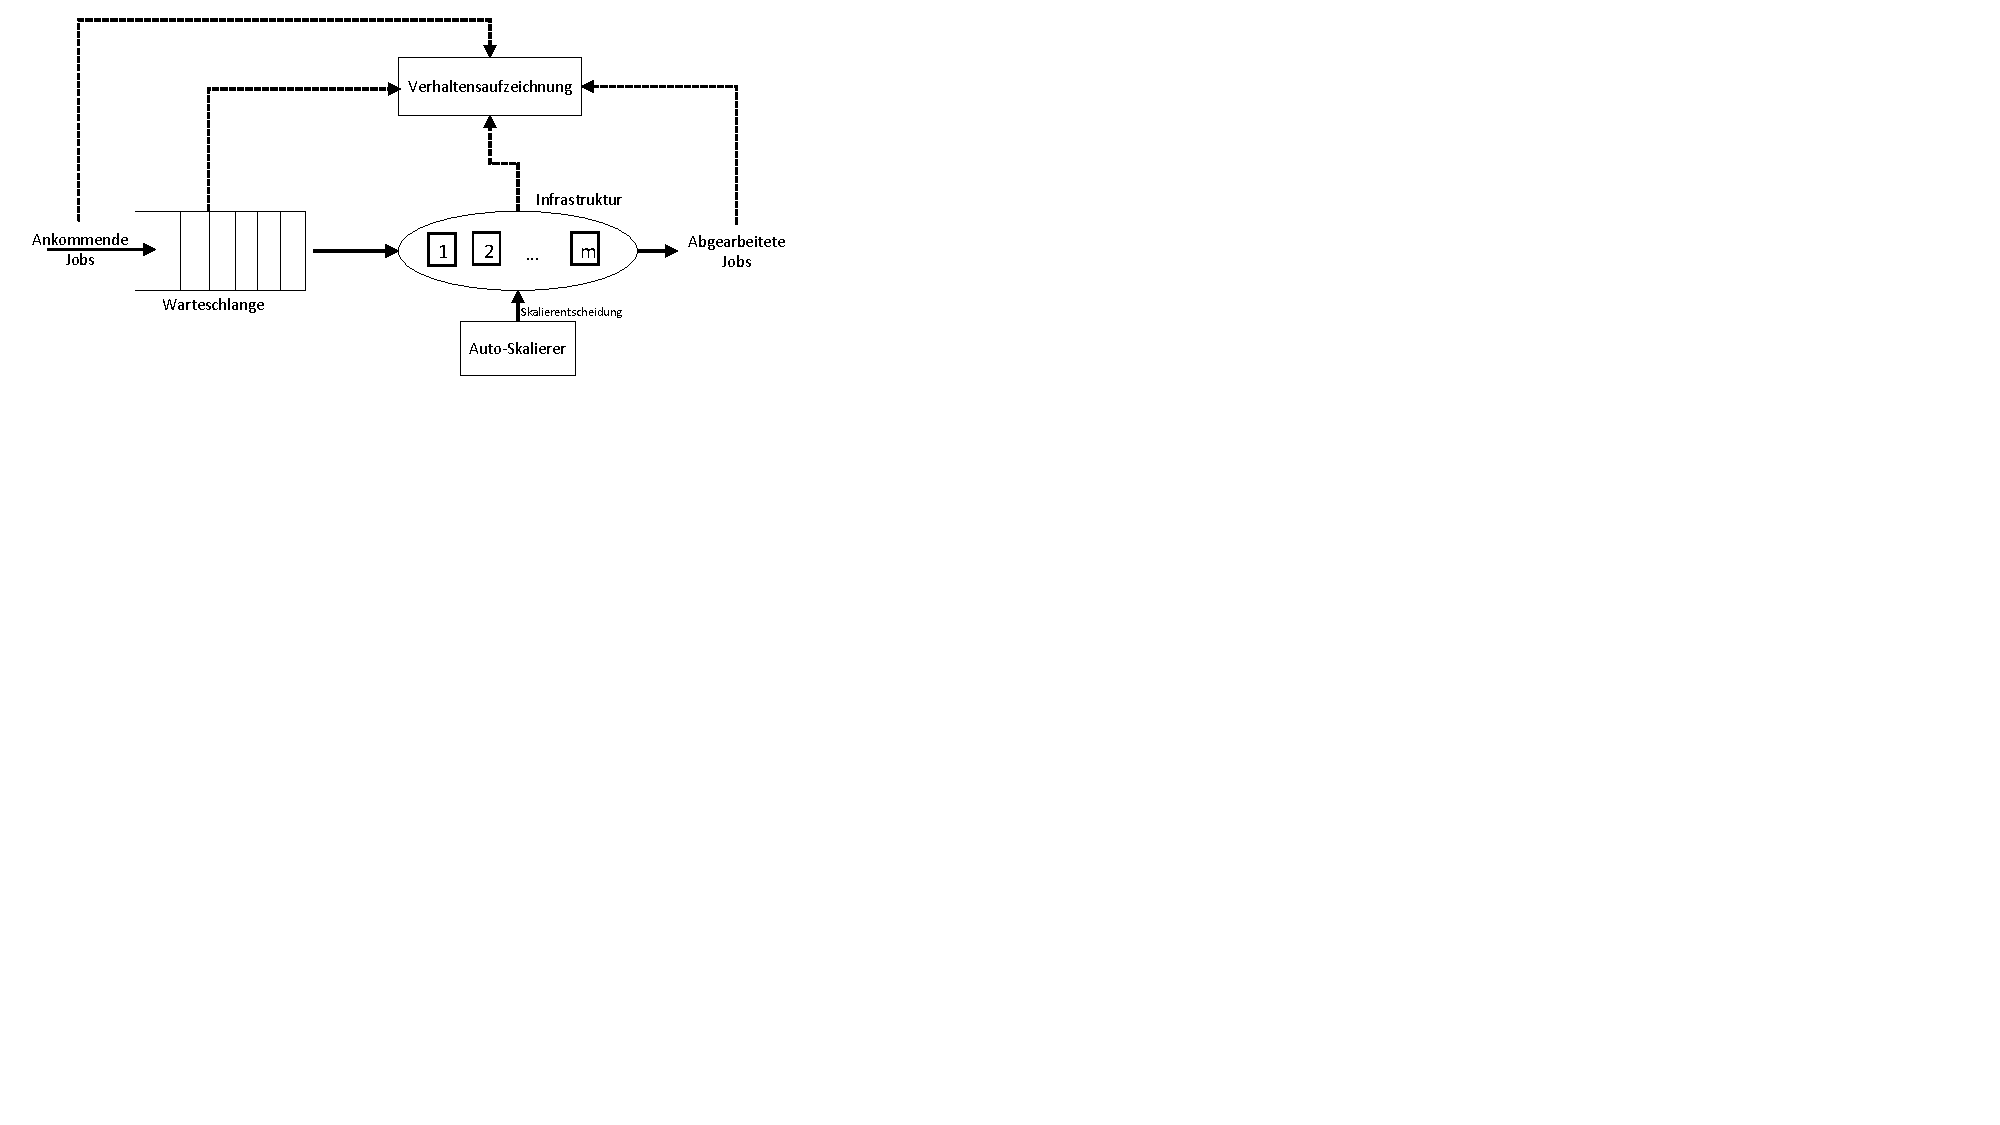
\includegraphics[width=\textwidth, trim={1cm 13cm 20cm 0cm}]{img/BasicIdea.pdf}
	\caption{Grundlegende Idee der Testbench}
	\label{fig:BasicIdea}
\end{figure}

\noindent
Zu einem Zeitpunkt \textit{t} erreicht eine (durch die gegebene Workload spezifizierte) Menge an Jobs das System und wird in der Warteschlange, die als Puffer fungiert, eingereiht. Die Infrastruktur wird durch eine Menge an Virtuellen Maschinen (\textit{VMs}) repräsentiert. Jede VM ist in der Lage in einer Zeiteinheit eine gewisse Menge an Jobs abzuarbeiten. Die Infrastruktur kann also pro Zeiteinheit eine durch die VMs definierte Menge an Jobs aus der Warteschlange nehmen und verarbeiten. Falls die Menge an ankommenden Jobs größer ist, als die Kapazität der Infrastruktur, so wird die Menge an wartenden Jobs in der Warteschlange größer. Diese Menge reduziert sich erst dann, wenn die Kapazität größer ist als die Last, wenn also entweder die Last unter dieses Level sinkt, oder aber die Kapazität durch eine Skalierentscheidung ausreichend vergrößert wird.\\
Allgemein ist die Testbench parametrisierbar. Beispielsweise soll die Warteschlangengröße und die Menge an maximal hinzuzufügenden VMs begrenzt sein. Weiterhin ist die Zeit zwischen Ankunft eines Jobs und dessen Abarbeitung in der Realität nicht gleich null. Diese und weitere Parameter können dynamisch konfiguriert werden, sodass nicht nur der Auto-Skalierer unter verschiedenen Lastbedingungen getestet werden kann, sondern auch auf unterschiedlich konfigurierten Infrastrukturen. \\
Um eine Skalier-Entscheidung treffen zu können, muss der Auto-Skalierer (je nach Typ) diverse Metriken der Infrastruktur oder der Warteschlange erheben, wie beispielsweise Länge der Warteschlange oder Auslastung der VMs. Dafür ist es notwendig, dass alle wichtigen Komponenten diese Metriken zu Verfügung stellen. \\
Um im Anschluss an eine Simulation den Auto-Skalierer bewerten zu können, wird der Zustand sämtlicher Komponenten zeitdiskret aufgezeichnet. Dabei werden Informationen wie Auslastung des Systems, Füllstand der Warteschlange, Durchsatz oder Wartezeiten im Puffer aufgezeichnet. Mittels dieser Daten kann dann das Verhalten des Auto-Skalierers, und damit seine Güte bestimmt werden.

\section{Übersicht}
\begin{itemize}
	\item \textbf{Kapitel \ref{ch:Architektur und Technologien}} beschreibt die verwendeten Technologien und die zugrundeliegende Architektur.
	
	\item In \textbf{Kapitel \ref{ch:Aufbau}} wird der Aufbau der Testbench auf Komponenten, bzw. Klassen-Ebene beschrieben. 
	\item Die Konfigurationsmöglichkeiten werden in \textbf{Kapitel \ref{ch:Konfiguration}} beschrieben.
	
	\item Abschließend wird die Applikation in \textbf{Kapitel \ref{ch:Evaluation} }evaluiert. Dafür werden Evaluationsaufbau- und Ergebnisse vorgestellt. Dieses Kapitel beendet die Dokumentation mit einer Zusammenfassung und einem Ausblick.
\end{itemize}

 



